\chapter{BACKGROUND RELATED WORK}
\label{ch:related}

\section{Background}
\label{rel:openflow}

Much of the work on the development of technologies for SDN is targeted at or 
inspired by OpenFlow: a specification describing the general architecture of SDN 
switches and the protocol that allows them to be remotely observed and controlled 
\cite{openflow_spec}. 
The key parts of the OpenFlow switch architecture, depicted in Figure \ref{fg:openflow_switch}, are a packet 
processing pipeline, an external software controller which sends and receives
OpenFlow messages, and ports. 

\begin{figure}[ht]
\centering
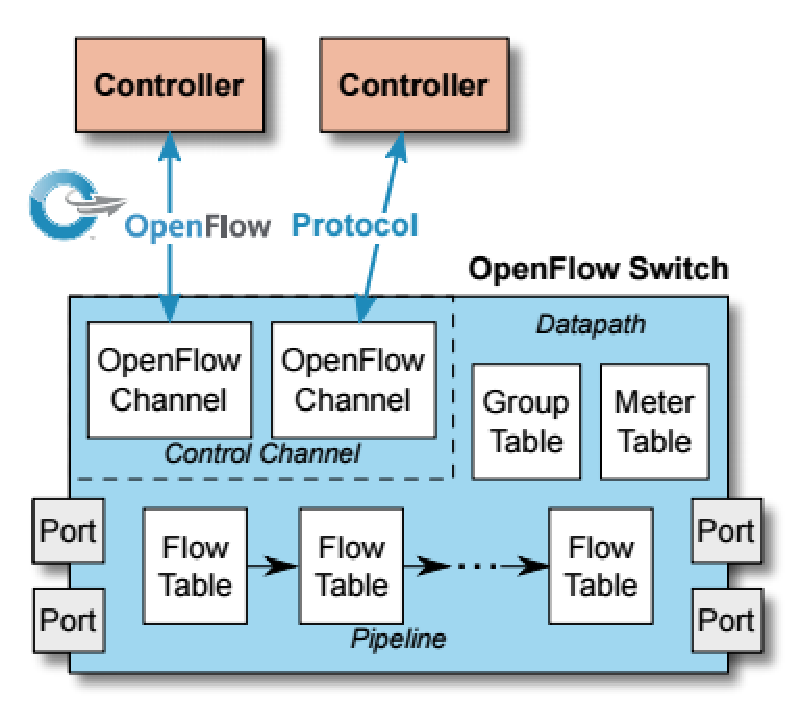
\includegraphics[scale=.5]{openflow}
\caption{The Openflow switch architecture is made up of ports, a pipeline,
and an external controller which uses OpenFlow messages to communicate. (Image Source: \cite{openflow_spec})}
\label{fg:openflow_switch}
\end{figure}

This is the architecture that most SDN researchers and vendors have focused on.
Though OpenFlow is widely accepted and has driven the majority of SDN research,
it has its flaws.
OpenFlow is protocol dependent and unscalable, a compromise which resulted from targeting non-programmable switch processors. However, modern programmable switch processors have rapidly caught up in performance \cite{bosshart2013forwarding}, making arbitrary packet processing more realizable. However, with OpenFlow, protocol independent research like Steve becomes artificially constrained.

Research into Steve used OpenFlow as a guidepost for what an abstract
packet processing machine might look like and what language features may be
necessary to support such a machine. However, by no means did this research
strictly adhere to OpenFlow principles or semantics.

The primary concept Steve takes from OpenFlow is the pipeline processing model.
An OpenFlow pipeline is defined as a sequence
of one or more \textit{flow tables} and a \textit{group table} which handle
packet lookups, decision making, and forwarding.

The Steve pipeline has two key differences.
The first difference is that
Steve's pipeline is protocol independent, whereas OpenFlow specifies a limited set of
supported protocol fields known as OXM fields.
Because Steve is protocol independent, its
pipeline model must contain a series of programmable decoders to extract fields
from user-specified header structures. 
OpenFlow does not mention decoding because
protocol dependent decoding is typically built into the switch.

The second difference is the actions used to modify the packet.
Steve flattens the instruction+action design of OpenFlow into
just actions. Steve actions are generic and may work with any protocol field, whereas OpenFlow only supports specific fields. It also provides action extensions to manipulate flow tables
which OpenFlow does not.
Steve also does away with OpenFlow's strict action set limitation, allowing any number of actions to be applied to a packet.

Since Steve focuses on programming a single switch that does not require distributed control, it does away with OpenFlow external controllers. 
Though the OpenFlow model provides
the benefit of supporting distributed control, sending messages
over a network is slow.
Instead, Steve chooses to leverage the power of the control plane which
resides on the same switch as the data plane.

%The abstract SDN switch proposed by OpenFlow is not completely adopted by
%the Freeflow runtime. Specifically, the remote OpenFlow controller was
%removed from the Freeflow switch model. It is not desirable to remote configure
%a switch for basic reactive programs. Sending messages to a controller through
%a wire is a prohibitively high-latency operation.
%Instead of communicating with a remote controller via messages, Freeflow uses an 
%internal (non-distributed) controller which executes Steve event handlers. 
%However, Steve is still capable of decoding OpenFlow messages like any other protocol
%if there is a need for a distributed controller.

%An OpenFlow pipeline is defined as a sequence
%of one or more \textit{flow tables} and a \textit{group table} which handle
%packet lookups, decision making, and forwarding. Steve's packet processing pipeline differs from the traditional OpenFlow
%semantics in a number of ways. First,
%Steve provides language features for a user to create flow tables and define
%their flow entries, but does not yet support group tables.
%
%Second, a Steve pipeline has more than \textit{just} flow tables. Steve
%pipelines will also have \textit{decoders} which may be interleaved between
%tables. Decoders define how fields get decoded (or parsed) and extracted. In
%most switches, decoding is handled by specialized hardware that deal with
%well-known headers. OpenFlow only supports certain fields from these headers,
%known as OXM fields. However, the Freeflow data plane is
%protocol oblivious, knowing nothing about any specific headers; therefore
%decoding must be an explicit user-defined stage of the pipeline. By extension,
%Steve does not, by default, support these OXM fields either.

%Third, the semantics for packet handling using an external controller are different. An OpenFlow controller is software used to control an OpenFlow switch. It will handle ``exceptional events'' such as inserting,
%removing, and updating flow entries or processing packets which the pipeline
%could not. However, Steve and Flowpath do not use nor expect an external
%OpenFlow controller nor do they use OpenFlow messages to communicate with that
%controller.

%Steve and Flowpath attempt to reduce the role of the controller. Controller
%functions, which would typically handle exceptional cases (such as table
%manipulation and un-handled packets), can be written in Steve using special
%event handler functions. These event handlers are executed by the data plane
%on a special internal Flowpath ``controller'' thread rather than relying on an
%external controller.

\section{Prior Steve Work}

Due to the sensitive nature of network applications, the program must be provably safe to execute.
Early development of Steve focused on the safe interpretation of packet memory as local objects.
Casey, et al., described the semantic constraints,
structural constraints (including buffer and view abstractions used by decoders), and 
safe access properties needed when working with packet headers as well as providing the early Steve language.
The Arbiter Framework was another language implementation that checked the correctness of data paths (pipelines) and ensured that they did not violate the 
capabilities of switches they ran on
\cite{arbiter}.

\section{SDN Programming Languages}

Many other projects have tackled the idea of an SDN programming language.
These languages may be further categorized into languages that program or configure
data plane elements, and languages which program the control plane or controller.

Languages which target the data plane all have the common idea of a pipeline.
These languages typically provide syntax for expressing packet decoding rules, table configuration,
and packet manipulation.
Controller languages tend to focus more on high-level, distributed control
of networks, designing network topology, and setting up forwarding policies
for an entire network.

Steve is unique in that it provides features for programming the data plane
and defines the reactive elements (i.e. event handlers) of the controller. However, since Steve
does not work with distributed control, it shares very little similarity with 
controller programming languages.

\subsection{SDN Data Plane Programming and Configuration Languages} \label{rel:p4}

P4 is the most popular protocol independent language for pipeline specification
 \cite{p4_spec, p4_spec2, p42014} on specialized ASIC switches.
P4 specifies a pipeline of programmable parsers (equivalent to Steve decoders) followed
by a series of match+action
tables (equivalent to flow tables). Parsing state is stored in a data structure
called a ``parsed representation.''

Protocol Oblivious Forwarding (POF) \cite{pof_fis, pof, pof_impl} provides a
an assembly-like instruction set for POF SDN switches.
The POF pipeline is a series of match tables which are also
responsible for decoding the fields they match on. 
The POF programming model uses metadata as a ``scratch pad'' for decoding fields,
requiring that the programmer represent fields as generic \textit{\{offset, length\}} pairs, 
known as ``search keys''. 
NetASM is an intermediate representation language for programmable data planes
\cite{shahbaz2015netasm}. It aims to solve the same issues as POF, but also provides a language that is target/device independent.

Steve is an approach between P4 and POF, but also attempts to
fill in their weaknesses. 
Steve's pipeline specification syntax is similar to P4.
P4's high-level, abstract syntax is easy to write and understand. 
In contrast, POF's instruction set (POF-FIS) \cite{pof_fis} is too
concrete, difficult to comprehend, and has no additional language
abstractions to ensure program safety.
POF search keys are particularly error prone because its not easy
for a programmer count field offsets manually.

However, Steve's abstract pipeline and decoding model is closer to POF's.
Steve decoders are placed between tables so fields are only decoded
as needed. This is similar to how POF tables extract their own fields.
Similarly, Steve uses POF's search key format for representing extracted fields, but the compiler generates the keys rather than the programmer.
The benefit of POF's decoding model is granular control over which fields from a header get extracted.
P4, on the other hand, extracts all header fields up-front, which wastes 
valuable processing time if those fields are not needed.
Also unlike P4, Steve allows the user to specify the complete pipeline logic, including pipeline composition, flow entry definitions, and flow entry insertion/removal. Because of this, the Steve compiler is able to reason about the safety of all flow entries which could ever exist and all potential execution paths that may exist at runtime.


%Essentially, fields only get extracted as they are needed, right before matching
%against a given table.

%Steve is a language for modifying the packet processing and forwarding functionality of a data plane. Steve is \textit{protocol oblivious}, meaning it does not by default
%know of any well-known network protocols (IPv4, IPv6, TCP, etc). Instead, it
%provides language features for programmers to deal with any protocol, making the
%language more scalable for future protocols. Other SDN languages are pursuing
%these idea as well.
%
%The P4 language \cite{p4_spec, p4_spec2, p42014} is another high-level language for
%defining protocol oblivious packet processing pipelines. It is probably the
%most widely adopted SDN language. P4 allows users to define packet headers,
%packet parsers and
%match+action tables (which are equivalent to OpenFlow flow tables). Parsers are
%used to extract entire headers and store them in a "parsed representation"
%before entering pipeline processing. When the packet enters the pipeline,
%match+action tables match against fields in the parsed representation and
%perform actions on matched packets.
%
%Protocol-Oblivious Forwarding (POF) \cite{pof_fis, pof, pof_impl} is another
%project also tackling the problem of protocol oblivious pipeline processing. POF
%is a very low-level, assembly-like, instruction set. The POF instruction
%set gives the programmer very fine-grained control of which fields get parsed.
%The POF programming model uses metadata as a "scratch pad" for parsing fields,
%requiring that the
%programmer represent fields as generic \{offset, length\} pairs, known as
%"search keys". When performing table matching, a programmer specifies
%an array of these search keys to match against the flow table.
%Essentially, fields only get extracted as they are needed, right before matching
%against a given table.
%
%POF also supports additional actions that allow the data plane to manipulate
%flow tables. This includes adding, removing, and updating flow
%entries. Though these actions are traditionally left up to the controller, they
%are useful because they reduce the load on the controller and provide
%flexibility to the data plane. This feature is notably absent from other SDN
%languages.
%
%The POF instruction set is difficult to write in and does not have the safety
%guarantees of a higher level language. The programmer is burdened with the
%error-prone task of parsing by manually specifying which bits comprise a fields.
%A high level language compiling into POF instructions would thus be ideal.
%
%Steve tries to take the best of both worlds. Steve can define decoding functions
%similar to P4 parsers, with the added benefit of allowing the programmer to only
%extract the fields they need, reducing the amount of time needed to parse
%overall. The \{offset, length\} pairs describing each field get generated by the
%Steve compiler rather than being manually written by the programmer, thus
%reducing
%the risk for error. Steve decoders may also be interleaved between tables,
%meaning fields can be extracted, as needed, right before table matching like
%POF. Like P4,
%Steve decoding can also happen all at once "up-front," before any table
%matching.
%It is up to the programmer to decide which is better. This makes Steve
%decoders a little more robust than either P4 or POF.
%
%Steve supports high-level definition of flow tables (or match+action tables in
%P4). Additionally, Steve also allows the programmer to define flow entries. This
%means the match field values and actions for each flow entry can be expressed
%within the language, allowing the Steve compiler to ensure safety and
%correctness guarantees over them. For example, adding a flow entry that causes
%an infinite loop is always prevented. This task is normally left up to the
%controller during runtime, which can be slow. Steve also supports instructions
%for adding and removing these flow entries from tables like POF.
%
%Unlike P4 and POF, Steve is not \textit{just} an SDN specific language; it is an
%extension to a general purpose language. It thus supports features like
%functions, function calls, lexical scoping, loops, conditional statements, and
%local/global variables. Steve also has support for types, arithmetic
%expressions, and comparison expressions. On top of that, it automatically links
%against the C Runtime Library, supports calls to external functions, and may be
%statically or dynamically linked against any library.
%
%Admittedly, P4 is a more mature language than Steve. P4 supports things like
%meters, variable sized fields, table matching methods (Steve only supports exact
%matching), and certain actions that Steve does not. P4 can also target more
%platforms than Steve, which currently only compiles into modules for Freeflow.
%POF also supports certain actions and table matching methods that Steve does not
%currently support.

\subsection{Data Plane Programming Libraries}
\label{rel:odp}

Data Plane Development Kit (DPDK) by Intel are software libraries in C for writing packet processing applications \cite{dpdk_webpage}. It improves packet processing speeds on Intel processors and NICs. DPDK provides a single platform (Intel processors) for performing all packet processing tasks, thus eliminating the need for specialized hardware.

Open Data Plane (ODP) is an open source API in C for developing data plane applications \cite{odp_webpage}. ODP provides application portability by providing a common set of APIs across multiple platforms and instruction set architectures.

\subsection{SDN Controller Programming Languages} \label{rel:frenetic}

The Frenetic project has produced a family of network programming
languages. Frenetic \cite{foster2011frenetic, foster2013frenetic} and Pyretic \cite{modularpyretic} are sister languages
that use SQL-like queries to classify packets and support a library for describing
packet forwarding policies over a collection of network switches. The goal is to
abstract away the difficulties of programming a centralized SDN controller.
NetCore is similarly a language for
generating classifiers from those policies \cite{monsanto2012netcore}. 
NetKAT is similar to NetCore except it uses Kleene algebra \cite{kozen2014netkat, anderson2014netkat} to prove the correctness of its policies.

\section{Packet Parsers and Header Specifications}

Other early DSLs focused on binary header specification languages which inspired Steve header specification syntax \cite{binpac, packet_types, datascript}.
Gibb, et al. described the design principles for parsing fields using header specifications
\cite{parser2013gibb}. Steve decoders may be described as a non-streaming programmable parsers according to Gibb, et al.
Some other examples of programmable packet parsers are Kangaroo \cite{kangaroo} and Berkley Packet Filter (BPF) \cite{bpf1993mccanne}. BPF also provides a language for filtering packets. It is possible for Steve programs to similarly act as a packet filter language rather than a packet forwarding language.

\section{Software Switches}
\label{rel:freeflow}

There exist a number of software switches which can be used to emulate or abstract SDN switch hardware.
Freeflow is an SDN software switch architecture developed
by Flowgrammable \cite{freeflow_software}. The Freeflow virtual machine (FFVM) 
provides a programmable, protocol oblivious, software data plane that 
supports multi-tenancy. Steve is
designed to generate code targeting the FFVM runtime environment. A Freeflow data 
plane loads Steve applications that act as its control plane and programs its packet processing pipeline.
P4 can similarly target a software switch called behavioral-model v2 (bmv2) \cite{bmv2_software}. 
Open vSwitch (OVS) is another SDN virtual, software switch which supports programmatic extensions \cite{ovs_man_page, ovs2009extending, ovs2013} and reconfiguration. Open vSwitch was designed to work in virtual environments and runs on the hypervisor.



